%%%%%%%%%%%%%%%%%%%%%%%%%%%%%%%%%%%%%%%%%
% Short Sectioned Assignment
% LaTeX Template
% Version 1.0 (5/5/12)
%
% This template has been downloaded from:
% http://www.LaTeXTemplates.com
%
% Original author:
% Frits Wenneker (http://www.howtotex.com)
%
% License:
% CC BY-NC-SA 3.0 (http://creativecommons.org/licenses/by-nc-sa/3.0/)
%
%%%%%%%%%%%%%%%%%%%%%%%%%%%%%%%%%%%%%%%%%

%----------------------------------------------------------------------------------------
%	PACKAGES AND OTHER DOCUMENT CONFIGURATIONS
%----------------------------------------------------------------------------------------

\documentclass[paper=a4, fontsize=11pt]{scrartcl} % A4 paper and 11pt font size

\usepackage[T1]{fontenc} % Use 8-bit encoding that has 256 glyphs
\usepackage{fourier} % Use the Adobe Utopia font for the document - comment this line to return to the LaTeX default
\usepackage[english]{babel} % English language/hyphenation
\usepackage{amsmath,amsfonts,amsthm} % Math packages

\usepackage{sectsty} % Allows customizing section commands
\usepackage[top=5em]{geometry}
\allsectionsfont{\centering \normalfont\scshape} % Make all sections centered, the default font and small caps

\usepackage{fancyhdr} % Custom headers and footers
\pagestyle{fancyplain} % Makes all pages in the document conform to the custom headers and footers
\fancyhead{} % No page header - if you want one, create it in the same way as the footers below
\fancyfoot[L]{} % Empty left footer
\fancyfoot[C]{} % Empty center footer
\fancyfoot[R]{\thepage} % Page numbering for right footer
\renewcommand{\headrulewidth}{0pt} % Remove header underlines
\renewcommand{\footrulewidth}{0pt} % Remove footer underlines
\setlength{\headheight}{5pt} % Customize the height of the header

\numberwithin{equation}{section} % Number equations within sections (i.e. 1.1, 1.2, 2.1, 2.2 instead of 1, 2, 3, 4)
\numberwithin{figure}{section} % Number figures within sections (i.e. 1.1, 1.2, 2.1, 2.2 instead of 1, 2, 3, 4)
\numberwithin{table}{section} % Number tables within sections (i.e. 1.1, 1.2, 2.1, 2.2 instead of 1, 2, 3, 4)

\setlength\parindent{0pt} % Removes all indentation from paragraphs - comment this line for an assignment with lots of text

\usepackage{mathtools}
\usepackage{amssymb}
\usepackage{gensymb}
\usepackage{chngcntr}
\usepackage{csquotes}
\usepackage{flexisym}
\usepackage{algorithm,algpseudocode}
\usepackage[toc,page]{appendix}
\newcommand\Mycomb[2][n]{\prescript{#1\mkern-0.5mu}{}C_{#2}}

\counterwithout{figure}{section}
%----------------------------------------------------------------------------------------
%	TITLE SECTION
%----------------------------------------------------------------------------------------

\newcommand{\horrule}[1]{\rule{\linewidth}{#1}} % Create horizontal rule command with 1 argument of height

\title{	
\normalfont \normalsize 
\textsc{Utah State University, Computer Science Department} \\ [25pt] % Your university, school and/or department name(s)
\horrule{0.5pt} \\[0.4cm] % Thin top horizontal rule
\huge CS 6670 Advanced Bioinformatics\\Assignment 3 \\ % The assignment title
\horrule{2pt} \\[0.5cm] % Thick bottom horizontal rule
}

\author{Gopal Menon} % Your name

\date{\normalsize\today} % Today's date or a custom date

\begin{document}

\maketitle % Print the title

\begin{enumerate}

\item \textbf{Biological Problem Description and Motivation}

Regulatory motifs are sequences of nucleotides that lie upstream of genes in a DNA molecule \cite{pevzner}. Proteins known as transcription factors bind to these motifs and by doing so, encourage RNA polymerase to transcribe the downstream gene. Motif finding is the process of discovering such motifs without prior knowledge of what the motif looks like. The approach to motif finding is based on the assumption that frequent or rare words may correspond to regulatory motifs in DNA. If a word occurs considerably more frequently than expected, then it is more likely to be some sort of \enquote{signal}.

Since we may not know what a motif looks like, we cannot just do a search for a nucleotide sequence within a DNA sequence. We need to be able to find out frequently occurring nucleotide sequences that may indicate a regulatory motif. A further complication is that some regulatory motifs may have mutations at some nucleotide locations and we still need to be able to find them.

\item \textbf{Problem Definition}

\begin{figure}[!h]
\centering
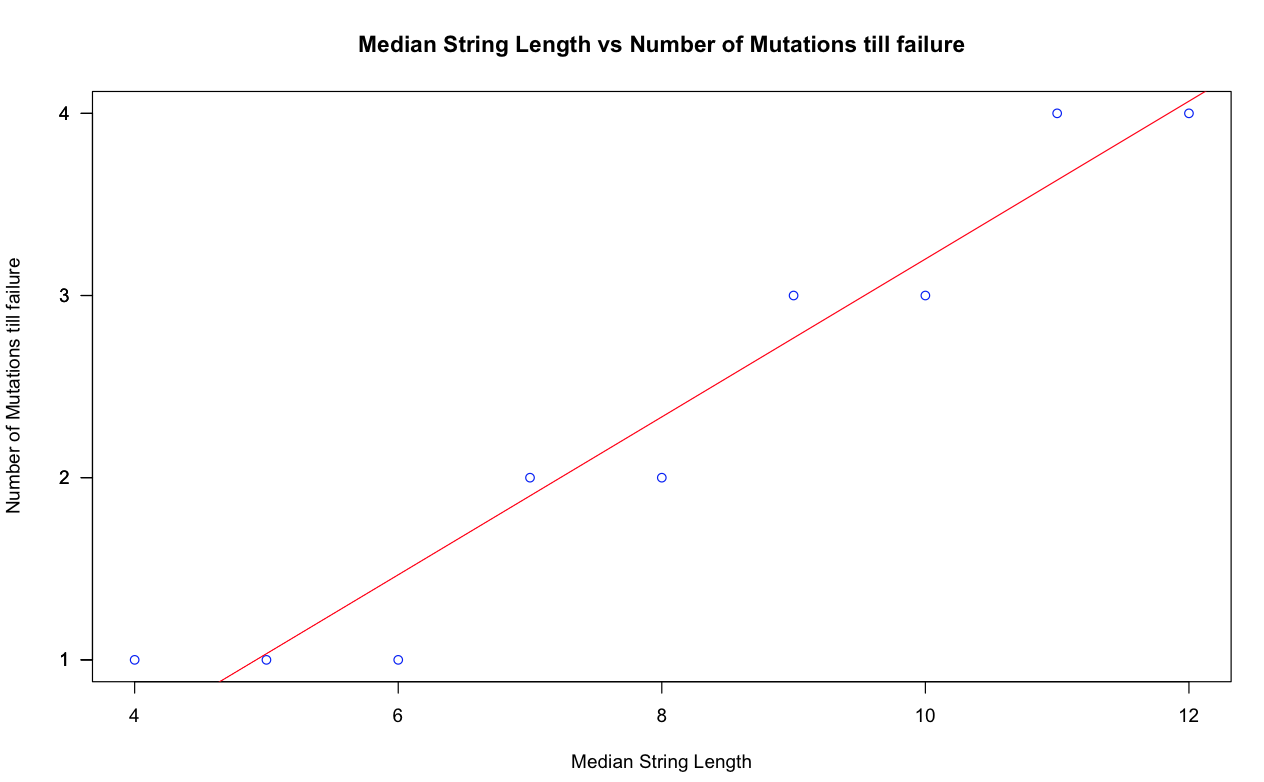
\includegraphics[width=6.75in]{Figures/MedianStringLenVsMutations.png}
\caption{Median String Length vs Number of Mutations till failure}
\label{MedStrLenVMutations}
\end{figure}

\begin{figure}[h]
\centering
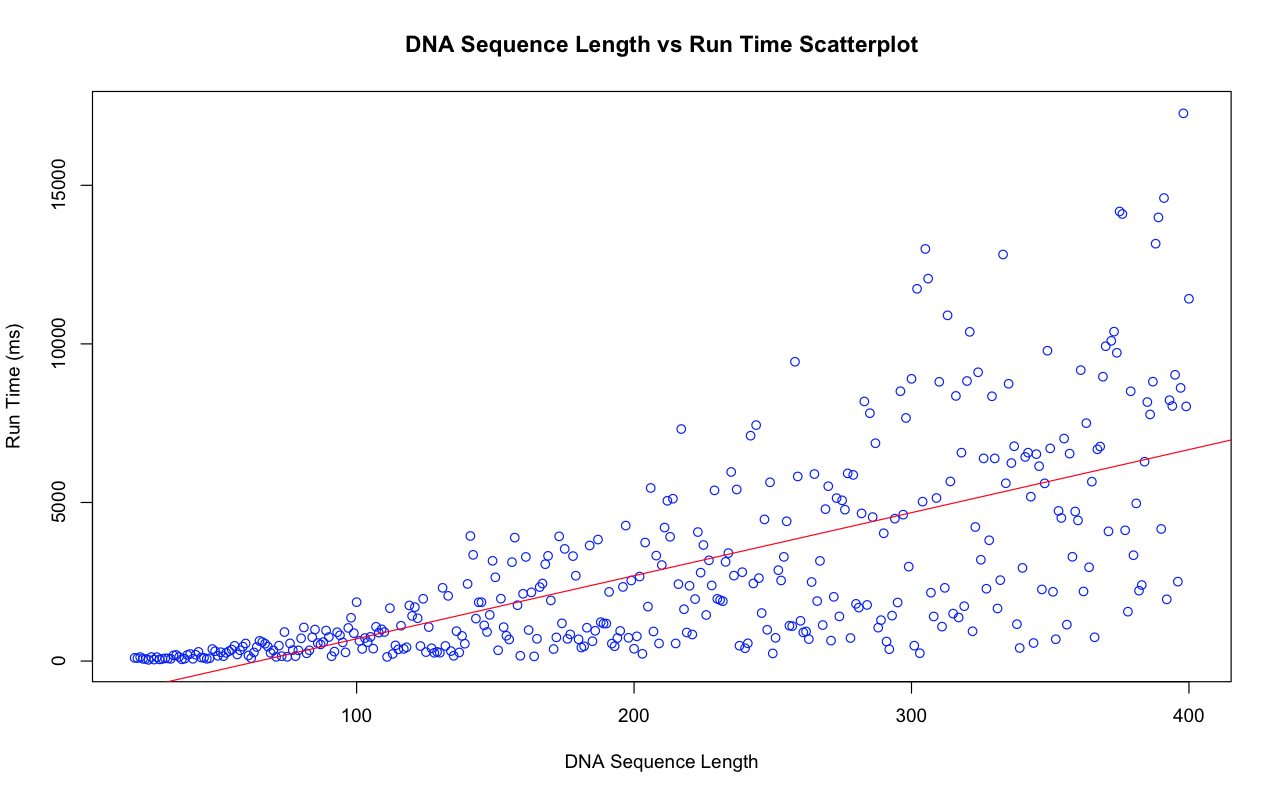
\includegraphics[width=6.75in]{Figures/DNASeqLengthVsRunTimeScatterplot.png}
\caption{DNA Sequence Length vs Run Time Scatterplot}
\label{SeqLenVRunTime}
\end{figure}

\begin{figure}[h]
\centering
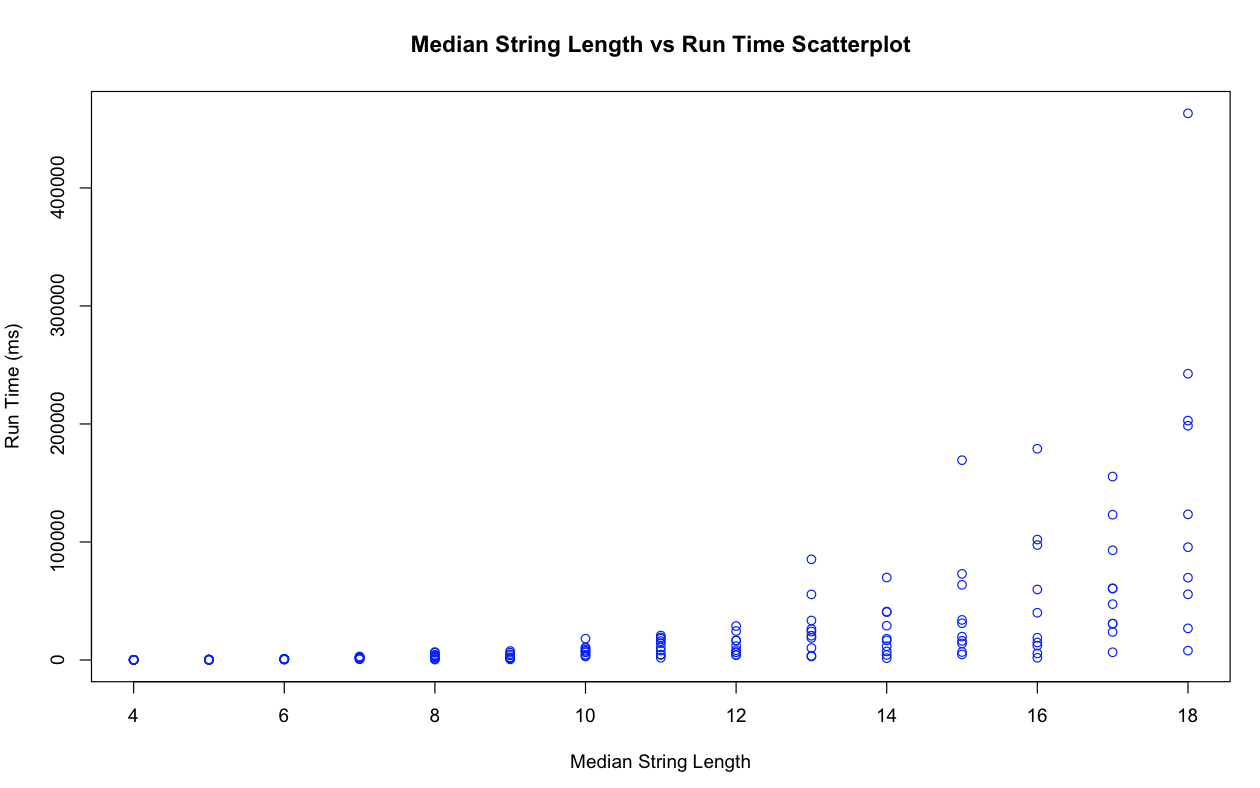
\includegraphics[width=6.75in]{Figures/MedianStringLengthvsRunTimeScatterplot.png}
\caption{Median String Length vs Run Time Scatterplot}
\label{MedLenVRunTime}
\end{figure}

\begin{figure}[h]
\centering
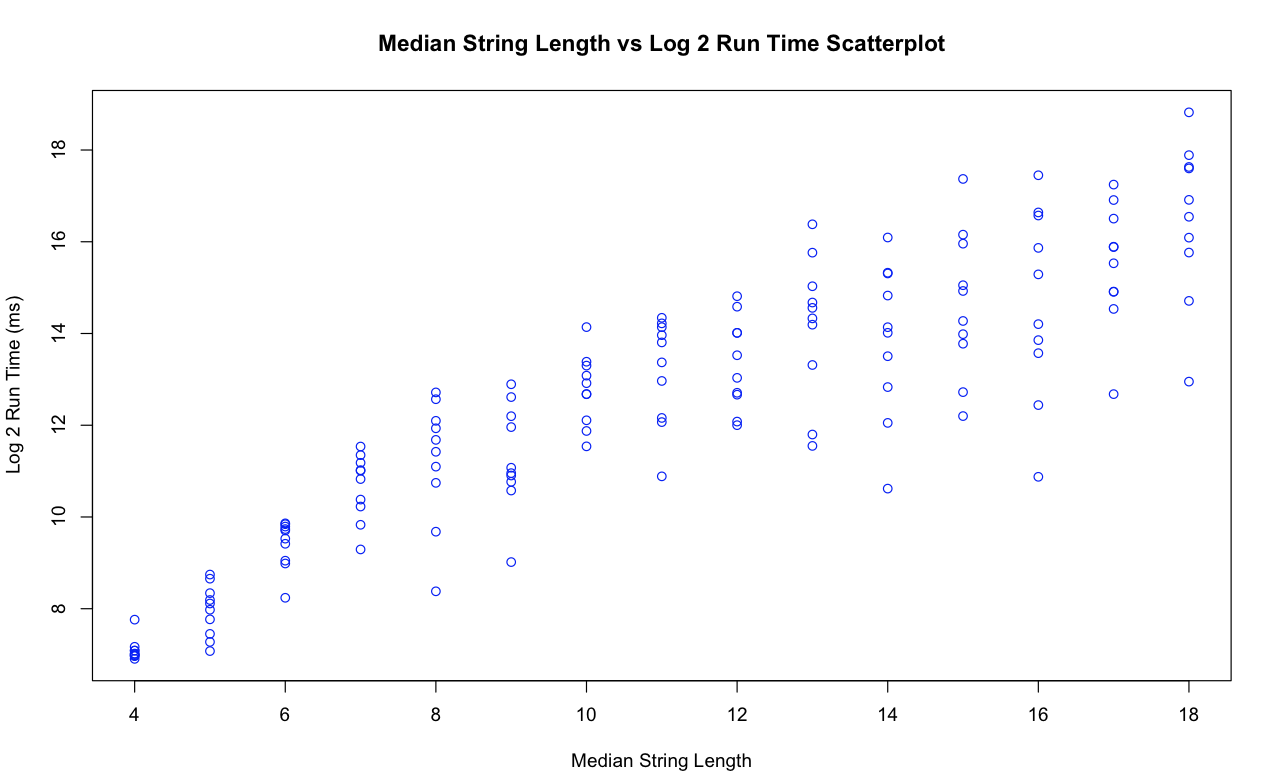
\includegraphics[width=6.75in]{Figures/MedianStringLengthvsLog2RunTimeScatterplot.png}
\caption{Median String Length vs Run Time Scatterplot}
\label{MedLenVLog2RunTime}
\end{figure}

A formal problem definition is given below \cite{pevzner}:

\horrule{0.5pt} \\[0.4cm]
\textbf{Median String Problem:}

\textit{Given a set of DNA sequences, find a median string.}

\textbf{Input:} A $t \times n$ matrix DNA, and $L$, the length of the pattern to find.

\textbf{Output:} A string $v$ of $L$ nucleotides that minimizes $TotalDistance(v, DNA)$ over all strings of that length.

\horrule{0.5pt} \\[0.4cm]
In other words, given a set of $t$ DNA sequences of length $n$ and a target median string length of $L$, we need to find a median string $v$ of length $L$ nucleotides that minimizes $TotalDistance(v, DNA)$. Here $TotalDistance(v, DNA)$ is the smallest hamming distance between the median string and all possible starting points starting points in each of the DNA sequences. 

\begin{verbatim}  caggggcaggaagacagagcagctgacacttccagaaatagctggccaga
                  gtagtaa\end{verbatim}

In the above string of nucleotides (the longer one could be thought of as a DNA sequence and the shorter one as a potential median string), the hamming distance at the position shown will be the number of nucleotides that are different. We can slide the potential median string and find the smallest hamming distance between it and the DNA sequence. The total distance will be the sum of minimum hamming distances between the potential median string and all the DNA sequences. The string of length $L$ that minimizes the total distance will be median string.

A median string described above would indicate a regulatory motif and its mutations that occur more frequently than expected, in a DNA sequence.

\item \textbf{Results with Synthetic Data}

\begin{enumerate}

\item \textbf{Mutations till failure}

Figure \ref{MedStrLenVMutations} shows the trend for the median string length versus the number of mutations at which the system fails to find the inserted median string. The test was done with 25 DNA sequences each of length 200. The blue circles are the data points and the red line is the line of best fit. It shows that with increasing median string length it takes more mutations for the system to fail to find the same median string that was inserted.

\item \textbf{DNA Sequence Length vs Run Time}

Figure \ref{SeqLenVRunTime} shows the plot for DNA Sequence Length vs Run Time for finding a median string. The data was collected for DNA Sequence Length varying from 20 to 400 nucleotides, 25 DNA sequences and a median string length of 8 with no mutations. For each DNA Sequence Length we can see data points varying from low to high run times. The reason is that the median string is randomly generated and those median strings that are checked for first in the branch and bound, are found earlier. The red line is the line of best fit and it shows a linear increase in run time with DNA Sequence Length. 

\item \textbf{Median String Length vs Run Time}

Figures \ref{MedLenVRunTime} and \ref{MedLenVLog2RunTime} show the plots for median string length vs run time to find a median string. The only difference between the two is that Figure \ref{MedLenVLog2RunTime} has a logarithmic scale for the run time. The plot seems to indicate that the run time is exponential in the length of the median string. The reason is that the logarithmic plot shows a linear relation. 

\end{enumerate}

\item \textbf{Results with Real Data}

Here are the results for the target length and the corresponding median strings found when run on the human DNA.\\

\begin{tabular}{ | c | r |}
  \hline			
  Target Length & Median String found  \\
  \hline			
  10 & AAAATTCAAA  \\
  \hline			
  11 & CTCCTGACCTC  \\
  \hline			
  12 & TTTTGTATTTTT  \\
  \hline  
\end{tabular}

\end{enumerate}

\clearpage
%----------------------------------------------------------------------------------------
\begin{thebibliography}{9}

\bibitem{pevzner} 
Jones, Neil C., and Pavel Pevzner. \enquote{Regulatory Motifs in DNA Sequences.} \textit{An Introduction to Bioinformatics Algorithms}. Cambridge, MA: MIT, 2004. N. pag. Print.

\end{thebibliography}

\appendix
\section{\\Program Parameters} \label{App:AppendixA}

These are the run time parameters to be provided while running the program.\\

\begin{tabular}{ l | c | c | c | c | c | }
\cline{2-6}
  & \multicolumn{5}{| c |}{ Parameter Number} \\
  \hline			
  Usage &1 & 2 & 3 & 4 & 5 \\
  \hline			
  DNA sequences in .txt files &T &    &   &   &   \\
  \hline			
  Use Human DNA sequences  &H &    &   &   &   \\
  \hline			
  Use generated DNA sequences  &G & DNA Seq Len  &  \# of DNA Seq &  Median Str Len &  \# of mutations \\
  \hline			
  Repeat till median string not found  &F &    &   &   &   \\
  \hline			
  Runtime with DNA sequence length  &L &    &   &   &   \\
 \hline			
  Runtime with median string length  &M &    &   &   &   \\
   \hline  
\end{tabular}

\end{document}